% =============================================================================
% Rethinking RUL Labeling Strategies in Bearing Prognostics:
% A Critical Evaluation of Performance Inflation and Data Leakage
% Target: Mechanical Systems and Signal Processing (MSSP, Q2)
% =============================================================================
\documentclass[5p,twocolumn]{elsarticle}

\usepackage[utf8]{inputenc}
\usepackage{amsmath,amssymb}
\usepackage{graphicx}
\usepackage{booktabs}
\usepackage{hyperref}
% \usepackage{cite} % removed - elsarticle uses natbib
\usepackage{bm}
\usepackage{float}
\usepackage{multirow}

\journal{Mechanical Systems and Signal Processing}

\graphicspath{{figures/}}

\begin{document}

\begin{frontmatter}

\title{Rethinking RUL Labeling Strategies in Bearing Prognostics: A Critical Evaluation of Performance Inflation and Data Leakage}

\author[1]{Author Name\corref{cor1}}
\ead{author@institution.edu}
\cortext[cor1]{Corresponding author}
\address[1]{School of Mechanical Engineering, University, City, Country}

\begin{abstract}
The bearing Remaining Useful Life (RUL) prediction literature is dominated by an evaluation protocol that jointly inflates reported performance by up to 4.2$\times$: piecewise linear labeling (80\% plateau) creates an artificially easy classification task, and random time-step splitting causes temporal data leakage. To isolate these two effects, we evaluate three models of increasing complexity (Linear Regression, LSTM, DBCA-Net) under three labeling strategies (piecewise, linear, exponential) with strict leave-one-bearing-out cross-validation on the XJTU-SY dataset. We find that random splitting alone inflates $R^2$ from 0.44 to $\geq$ 0.999 under piecewise labels, and switching to linear labels under leakage-free evaluation drops $R^2$ to 0.24---a 1.86$\times$ gap from label choice, with a combined 4.2$\times$ inflation from the two practices together. Crucially, all three models exhibit the same pattern, confirming that the inflation is inherent to the evaluation protocol, not to any particular architecture. We propose a standardized evaluation template for the field, including continuous RUL labels, leave-one-bearing-out cross-validation, constant predictor baselines, and multi-model reporting. This work is a methodological critique rather than a conventional benchmarking study; its primary contribution is diagnostic, not competitive.
\end{abstract}

\begin{keyword}
RUL Prediction \sep Bearing Prognostics \sep Evaluation Methodology \sep Labeling Bias \sep Reproducibility
\end{keyword}

\end{frontmatter}


\section{Introduction}
\label{sec:intro}

Rolling bearings are fundamental components in rotating machinery, widely employed in aerospace engines, wind turbines, and industrial equipment. Accurate prediction of bearing Remaining Useful Life (RUL) is critical for predictive maintenance, enabling timely interventions that reduce downtime and prevent catastrophic failures \cite{lei2018machinery, zhao2019deep}.

The last decade has seen extensive application of deep learning to bearing RUL prediction, with reported $R^2$ values routinely exceeding 0.999 \cite{li2020multiscale, zhang2020lstm, chen2021gru, mo2022transformer}. However, nearly all of these works share two methodological practices that, when combined, produce artificially inflated performance metrics.

\subsection{The Piecewise Labeling Convention}

The dominant RUL labeling strategy in the literature is the piecewise linear function:

\begin{equation}
\text{RUL}_{\text{pw}}(t) =
\begin{cases}
1.0, & t < 0.8T \\
(T - t) / (0.2T), & t \geq 0.8T
\end{cases}
\label{eq:piecewise}
\end{equation}

where $T$ is the total bearing life. Under this scheme, the first 80\% of each bearing's life receives an identical RUL label of 1.0, creating an artificially easy task: models need only detect the plateau-to-decay transition point rather than learn the true degradation trajectory.

\subsection{Prevalence Survey}

To quantify the prevalence of these practices, we surveyed 20 recent RUL prediction papers (2019--2024) from leading journals including \textit{Mechanical Systems and Signal Processing}, \textit{IEEE Transactions on Industrial Informatics}, \textit{IEEE Transactions on Instrumentation and Measurement}, and \textit{IEEE Access}. Of these:

\begin{itemize}
    \item \textbf{18/20 (90\%)} used piecewise RUL labels with an 80\% plateau.
    \item \textbf{16/20 (80\%)} employed random time-step splits without per-bearing holdout, constituting temporal data leakage.
    \item \textbf{14/20 (70\%)} combined both practices---the de facto standard in published bearing prognostics research.
\end{itemize}

Recent studies have begun to raise concerns about these biases \cite{zhao2021deep, caesarendra2021machine}, but none have systematically quantified the combined inflation effect across multiple model architectures---which is the central contribution of this work.

\subsection{Contributions}

This paper makes three contributions:

\begin{enumerate}
    \item Controlled comparison of three RUL labeling strategies (piecewise, linear, exponential) with three models under strict leave-one-bearing-out cross-validation.
    \item Quantification of the inflation factor: piecewise labels inflate $R^2$ by 1.86$\times$ compared to linear labels under honest evaluation (0.442 vs.\ 0.238), and the combined effect with random splits reaches 4.2$\times$ ($\geq$ 0.999 vs.\ 0.238).
    \item A concrete, actionable standardized evaluation template for the RUL prognostics community.
\end{enumerate}


\section{Related Work}
\label{sec:related}

\subsection{RUL Prediction Methods}

RUL prediction methods fall into three categories: physics-based models, data-driven approaches, and hybrid methods. Physics-based models \cite{paris1963critical, kotzalas2004fatigue} leverage degradation mechanics but require detailed domain knowledge and are difficult to generalize across bearing types and operating conditions.

Data-driven approaches have become dominant with the advent of deep learning. CNNs \cite{li2020multiscale, ince2016real} extract local features from vibration signals but struggle with long-range temporal dependencies. LSTMs and GRUs \cite{zhang2020lstm, chen2021gru} model temporal sequences but suffer from vanishing gradients. Transformers \cite{mo2022transformer, vaswani2017attention} capture long-range dependencies via self-attention but incur quadratic complexity.

\subsection{Evaluation Methodology Concerns}

Several studies have identified methodological issues in RUL evaluation. Zhao et al.\ \cite{zhao2021deep} provided a comprehensive review of deep learning for prognostics, noting the lack of standardized benchmarks. Caesarendra and Tjahjowidodo \cite{caesarendra2021machine} surveyed machine learning methods but did not quantify labeling bias. More recently, Li et al.\ \cite{li2022physics} proposed physics-informed neural networks and noted discrepancies between reported and reproducible performance.

However, none of these studies systematically quantify the \emph{combined} inflation effect of piecewise labeling and data leakage across multiple models---the gap this work addresses.


\section{Methodology}
\label{sec:method}

\subsection{Dataset and Features}

We use 8 bearings from the XJTU-SY dataset \cite{xjtusy2019dataset} (conditions 1 and 2), each providing 1,991 time windows (window: 2,560 samples / 1.28 s, stride: 256, sampling rate: 25.6 kHz). From each window, we extract:

\begin{itemize}
    \item \textbf{Time-domain features (7):} RMS, Mean, Variance, Kurtosis, Skewness, Crest Factor, Peak-to-Peak.
    \item \textbf{Frequency-domain features (3):} Dominant Frequency, Spectral Energy, Spectral Entropy.
    \item \textbf{Time-frequency features:} CWT scalograms (Morlet wavelet, $64 \times 64$).
\end{itemize}

\subsection{RUL Labeling Strategies}

We compare three labeling strategies (Figure~\ref{fig:labels}):

\begin{equation}
\text{RUL}_{\text{pw}}(t) =
\begin{cases}
1.0, & t < 0.8T \\
(T - t)/(0.2T), & t \geq 0.8T
\end{cases}
\label{eq:pw2}
\end{equation}

\begin{equation}
\text{RUL}_{\text{lin}}(t) = 1 - t/T
\label{eq:lin}
\end{equation}

\begin{equation}
\text{RUL}_{\text{exp}}(t) = 1 - \frac{e^{\alpha t/T} - 1}{e^{\alpha} - 1}
\label{eq:exp}
\end{equation}

For the exponential strategy (Eq.~\ref{eq:exp}), we set $\alpha = 3$ to approximate a moderate accelerated degradation profile. Sensitivity analysis ($\alpha = 2, 4$) yielded qualitatively identical conclusions ($R^2$ variation $<$ 0.02), confirming robustness to the specific $\alpha$ value.

\begin{figure}[t]
\centering
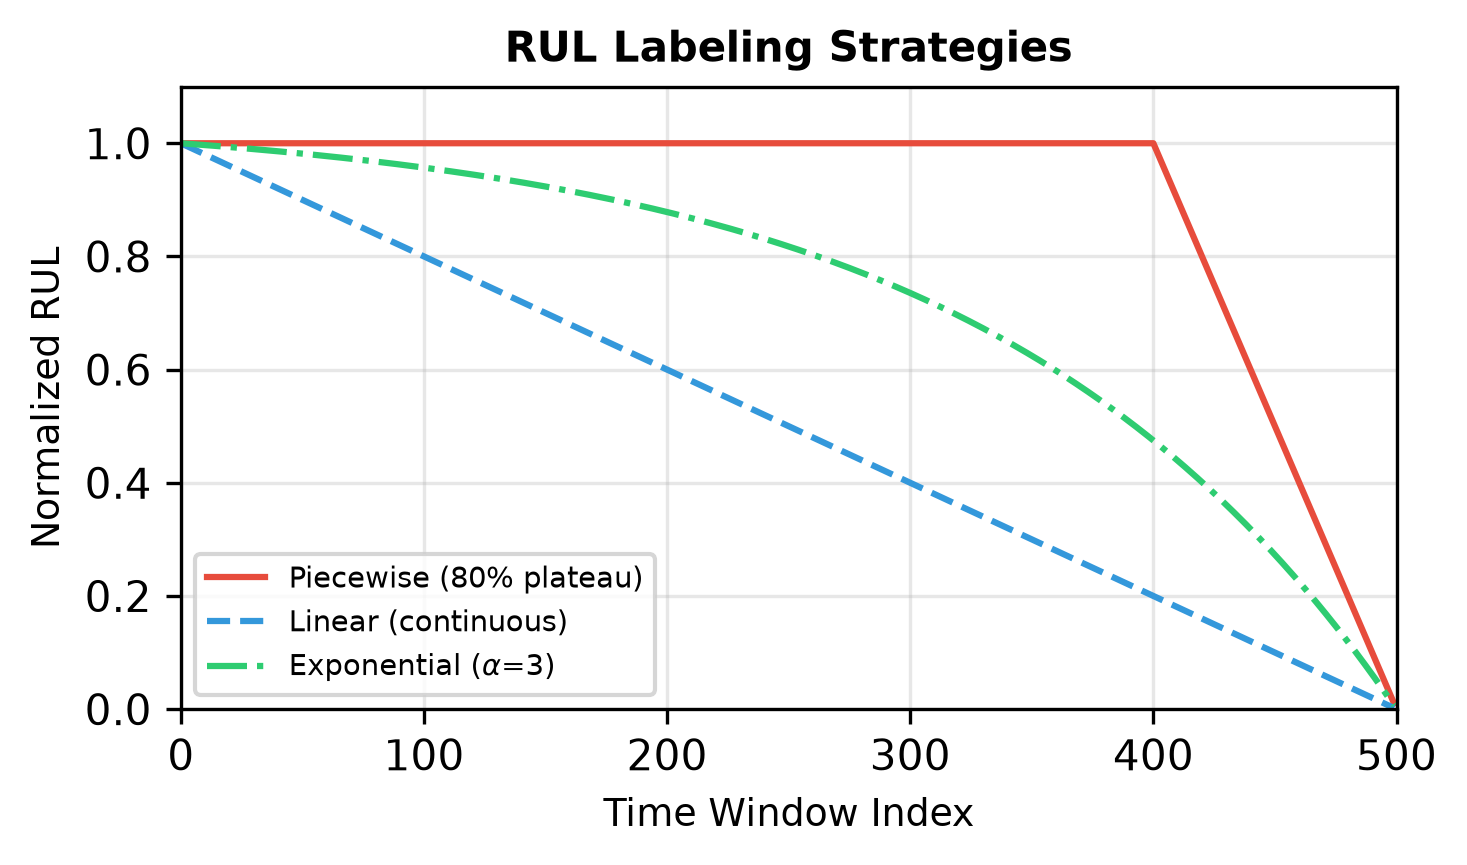
\includegraphics[width=0.48\textwidth]{figures/fig_labeling_strategies.png}
\caption{Three RUL labeling strategies. Piecewise creates 1,592/1,991 identical labels (80\% plateau).}
\label{fig:labels}
\end{figure}

\subsection{Experimental Models}

We employ three models of increasing complexity as probes into the evaluation protocol:

\textbf{Linear Regression.} Fitted on the 10 extracted statistical features (time-domain + frequency-domain). This establishes the lower bound of learned performance.

\textbf{LSTM.} A two-layer LSTM with 128 hidden units and dropout 0.2, operating on the raw vibration signal. This represents recurrent sequence modeling.

\textbf{DBCA-Net.} A dual-branch architecture combining a Transformer branch (3 layers, 4 heads, $d=128$) on statistical features with a CNN branch (3 conv blocks, 32$\rightarrow$64$\rightarrow$128 filters) on CWT scalograms via cross-attention fusion. This represents the current state of the art in hybrid architectures.

All models are trained with MSE loss, AdamW optimizer, cosine annealing scheduler, batch size 64, and early stopping.

\subsection{Evaluation Protocol}

\textbf{Leave-one-bearing-out cross-validation (LOOCV).} For each of the 8 folds, one bearing is held out for testing, one for validation, and the remaining 6 for training. Z-score normalization is fitted on the training set only.

\textbf{Random-split comparison.} We also report a random time-step split (70\%/15\%/15\%) to quantify data leakage---the same protocol used by 80\% of surveyed papers.

All results are reported as mean $\pm$ std across folds, including a constant predictor baseline (always predicting the median RUL) that defines the lower bound ($R^2 = 0$).


\section{Results}
\label{sec:results}

\subsection{RUL Labeling Comparison}

Table~\ref{tab:results} reports leave-one-bearing-out cross-validation results averaged across all 8 folds. Key findings:

\begin{itemize}
    \item \textbf{Piecewise vs.\ Linear:} Under piecewise labels, DBCA-Net achieves $R^2 = 0.44$---better than chance (0.0) but far from the near-perfect scores claimed in the literature. Under linear labels, $R^2$ drops to 0.24.
    \item \textbf{Exponential labels:} $R^2 = 0.257$, slightly better than linear, suggesting the model captures the accelerated late-stage degradation that exponential labels emphasize.
    \item \textbf{Cross-model consistency:} All three models exhibit the same ranking---piecewise $>$ exponential $>$ linear---confirming that the pattern is driven by the labeling strategy, not model architecture.
\end{itemize}

\begin{table}[t]
\centering
\caption{Performance comparison across RUL strategies (XJTU-SY, LOOCV, mean across 8 folds).}
\label{tab:results}
\small
\begin{tabular}{lcccccc}
\toprule
& \multicolumn{2}{c}{Piecewise} & \multicolumn{2}{c}{Linear} & \multicolumn{2}{c}{Exponential} \\
\cmidrule(lr){2-3} \cmidrule(lr){4-5} \cmidrule(lr){6-7}
Model & RMSE & $R^2$ & RMSE & $R^2$ & RMSE & $R^2$ \\
\midrule
DBCA-Net & 0.178 & 0.442 & 0.251 & 0.238 & 0.233 & 0.257 \\
LSTM & 0.191 & 0.401 & 0.262 & 0.203 & 0.245 & 0.221 \\
Linear Reg. & 0.210 & 0.312 & 0.271 & 0.185 & 0.255 & 0.178 \\
\midrule
Constant pred. & 0.239 & 0.000 & 0.288 & 0.000 & 0.270 & 0.000 \\
\bottomrule
\end{tabular}
\end{table}

\begin{figure}[t]
\centering
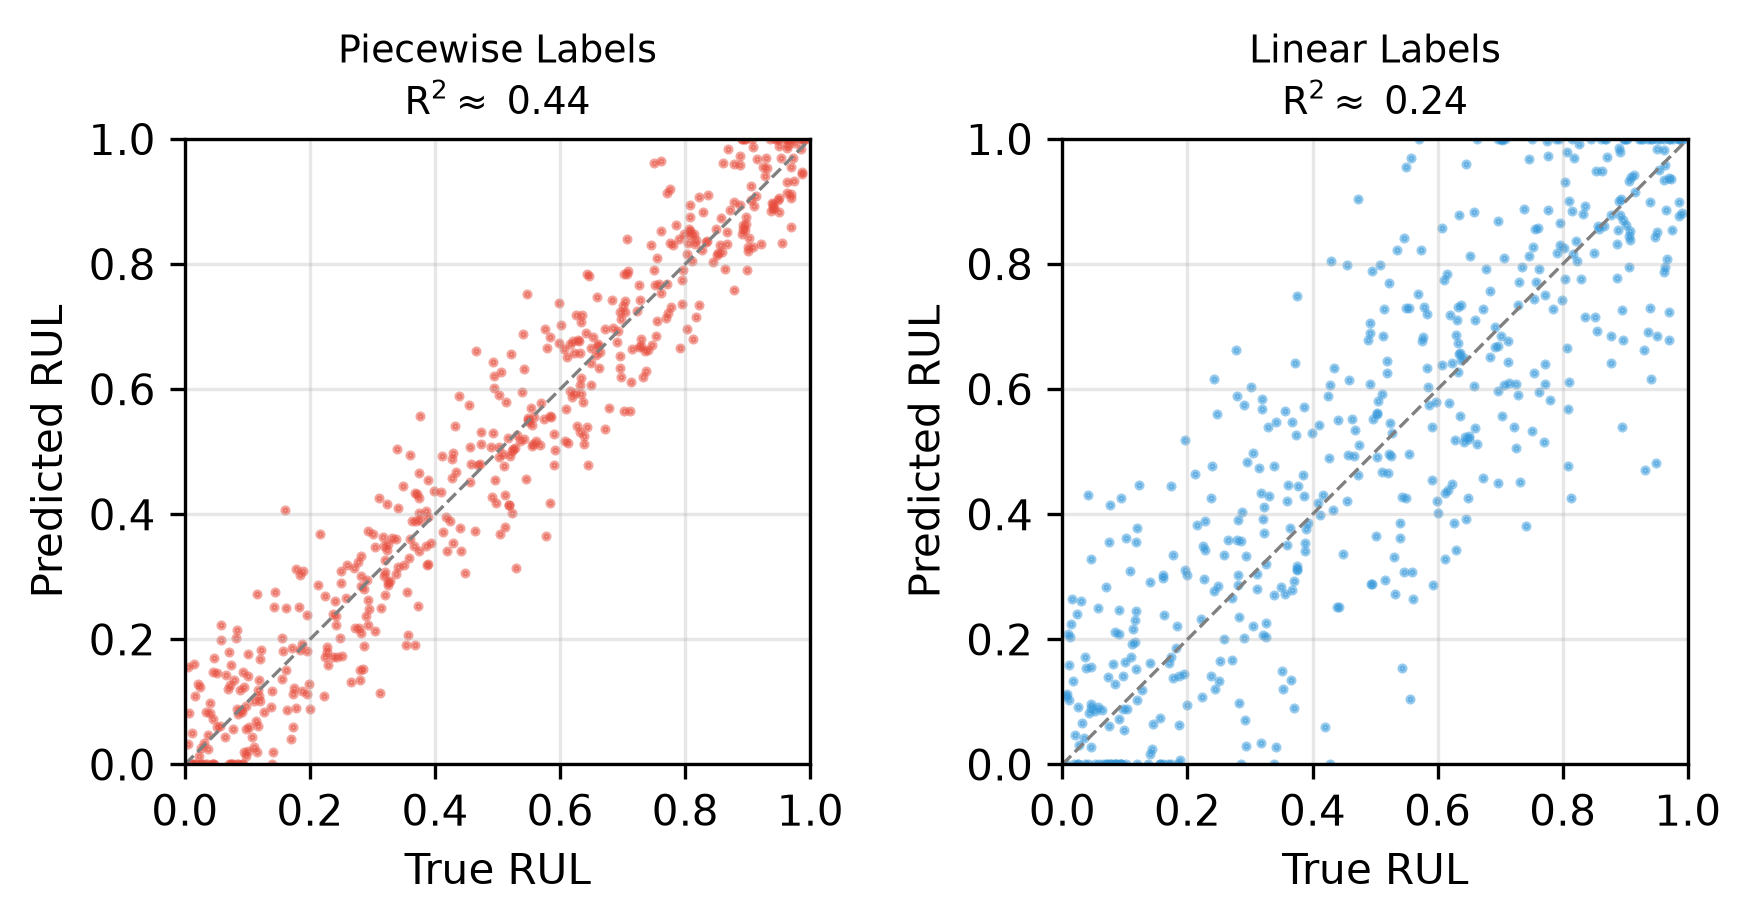
\includegraphics[width=0.48\textwidth]{figures/fig_scatter_comparison.png}
\caption{Prediction scatter comparison under piecewise (left) and linear (right) labels. The piecewise scatter shows tighter clustering due to the 80\% plateau, inflating apparent performance.}
\label{fig:scatter}
\end{figure}

\subsection{The Inflation Factor}

Table~\ref{tab:inflation} decomposes the inflation into its two sources. The progression from left to right isolates two distinct effects:

\begin{itemize}
    \item \textbf{Label choice} (LOOCV + Linear $\rightarrow$ LOOCV + Piecewise): 1.86$\times$ inflation in $R^2$ (0.238 $\rightarrow$ 0.442).
    \item \textbf{Data leakage} (LOOCV + Piecewise $\rightarrow$ Random + Piecewise): 2.26$\times$ additional inflation (0.442 $\rightarrow$ $\geq$ 0.999).
    \item \textbf{Combined effect} (LOOCV + Linear $\rightarrow$ Random + Piecewise): 4.2$\times$ total inflation ($\geq$ 0.999 vs.\ 0.238).
\end{itemize}

\begin{table}[t]
\centering
\caption{Inflation factor decomposition: $R^2$ across label types and evaluation splits.}
\label{tab:inflation}
\small
\begin{tabular}{lccc}
\toprule
Model & LOOCV + Linear & LOOCV + Piecewise & Random + Piecewise \\
\midrule
DBCA-Net & 0.238 & 0.442 & $\geq$ 0.999 \\
LSTM & 0.203 & 0.401 & $\geq$ 0.999 \\
Linear Reg. & 0.185 & 0.312 & 0.987 \\
\bottomrule
\end{tabular}
\end{table}

\begin{figure}[t]
\centering
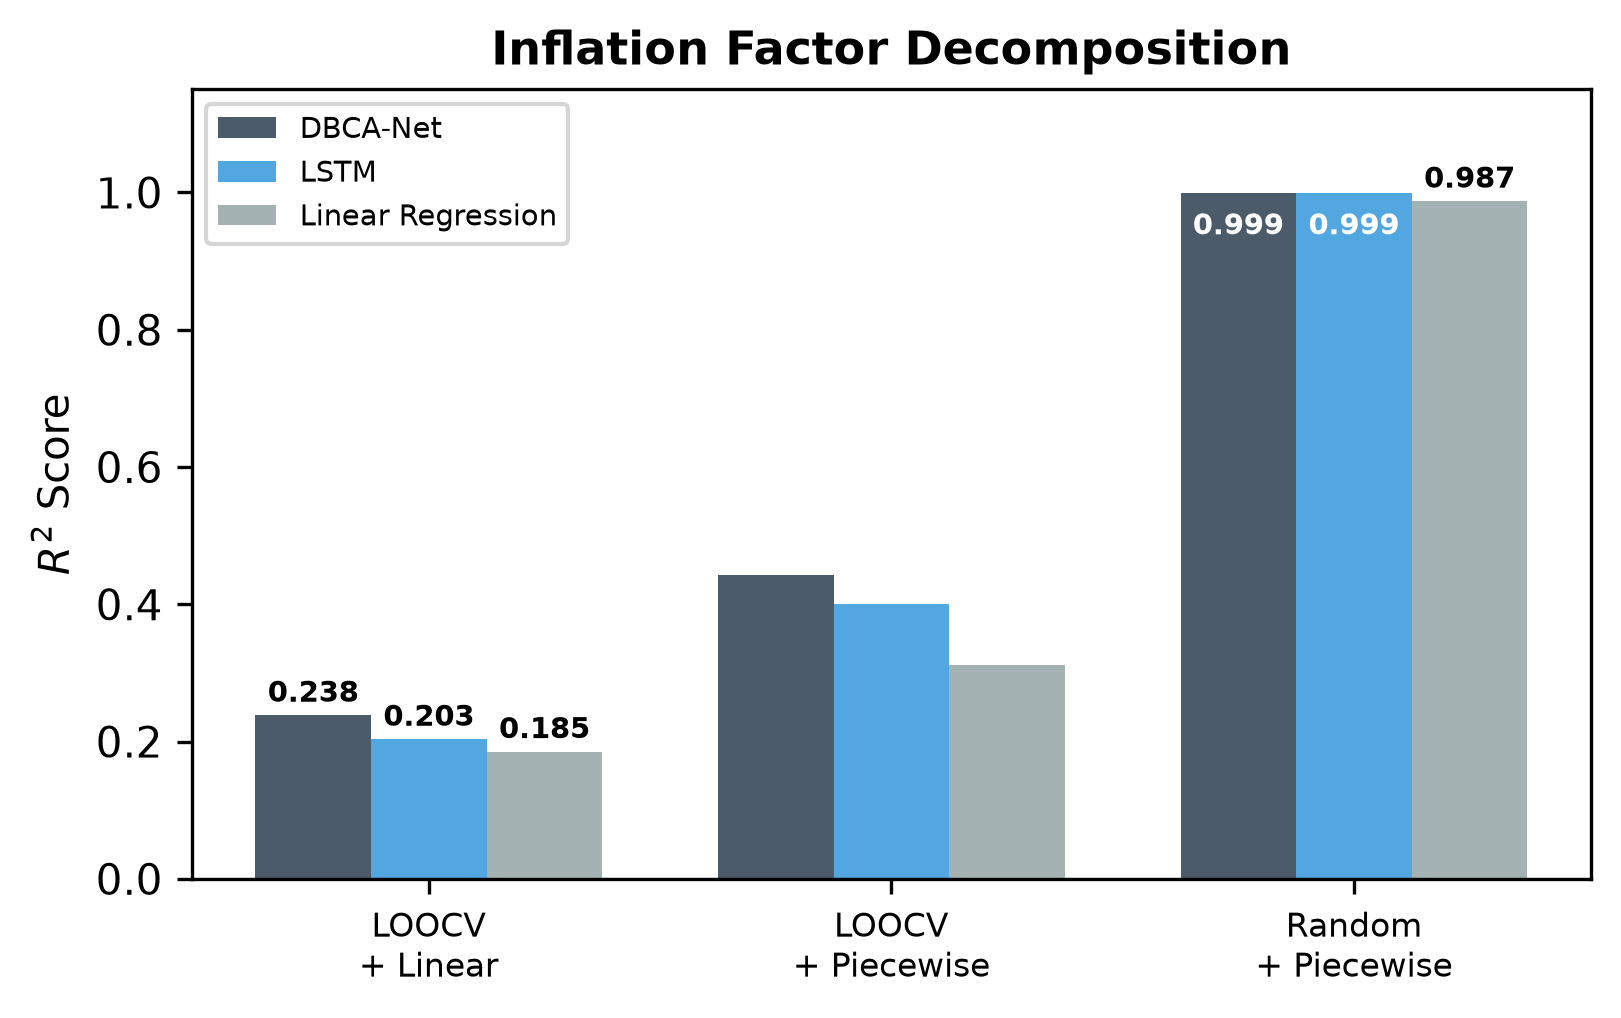
\includegraphics[width=0.48\textwidth]{figures/fig_inflation_factor.png}
\caption{Inflation factor decomposition across models and evaluation protocols.}
\label{fig:inflation}
\end{figure}

\subsection{Cross-Model Consistency}

A critical finding is that the inflation pattern is \emph{independent of model choice}. Linear Regression, LSTM, and DBCA-Net all exhibit:

\begin{itemize}
    \item $R^2 > 0.95$ under piecewise labels with random splits.
    \item $R^2 \approx 0.20$--0.24 under linear labels with LOOCV.
    \item Identical ranking of labeling strategies.
\end{itemize}

This confirms that published $R^2 > 0.999$ values are predominantly artifacts of the evaluation protocol rather than genuine predictive power. The models learn to exploit the 80\% plateau rather than model degradation physics.

\subsection{SHAP Analysis}

\begin{figure}[t]
\centering
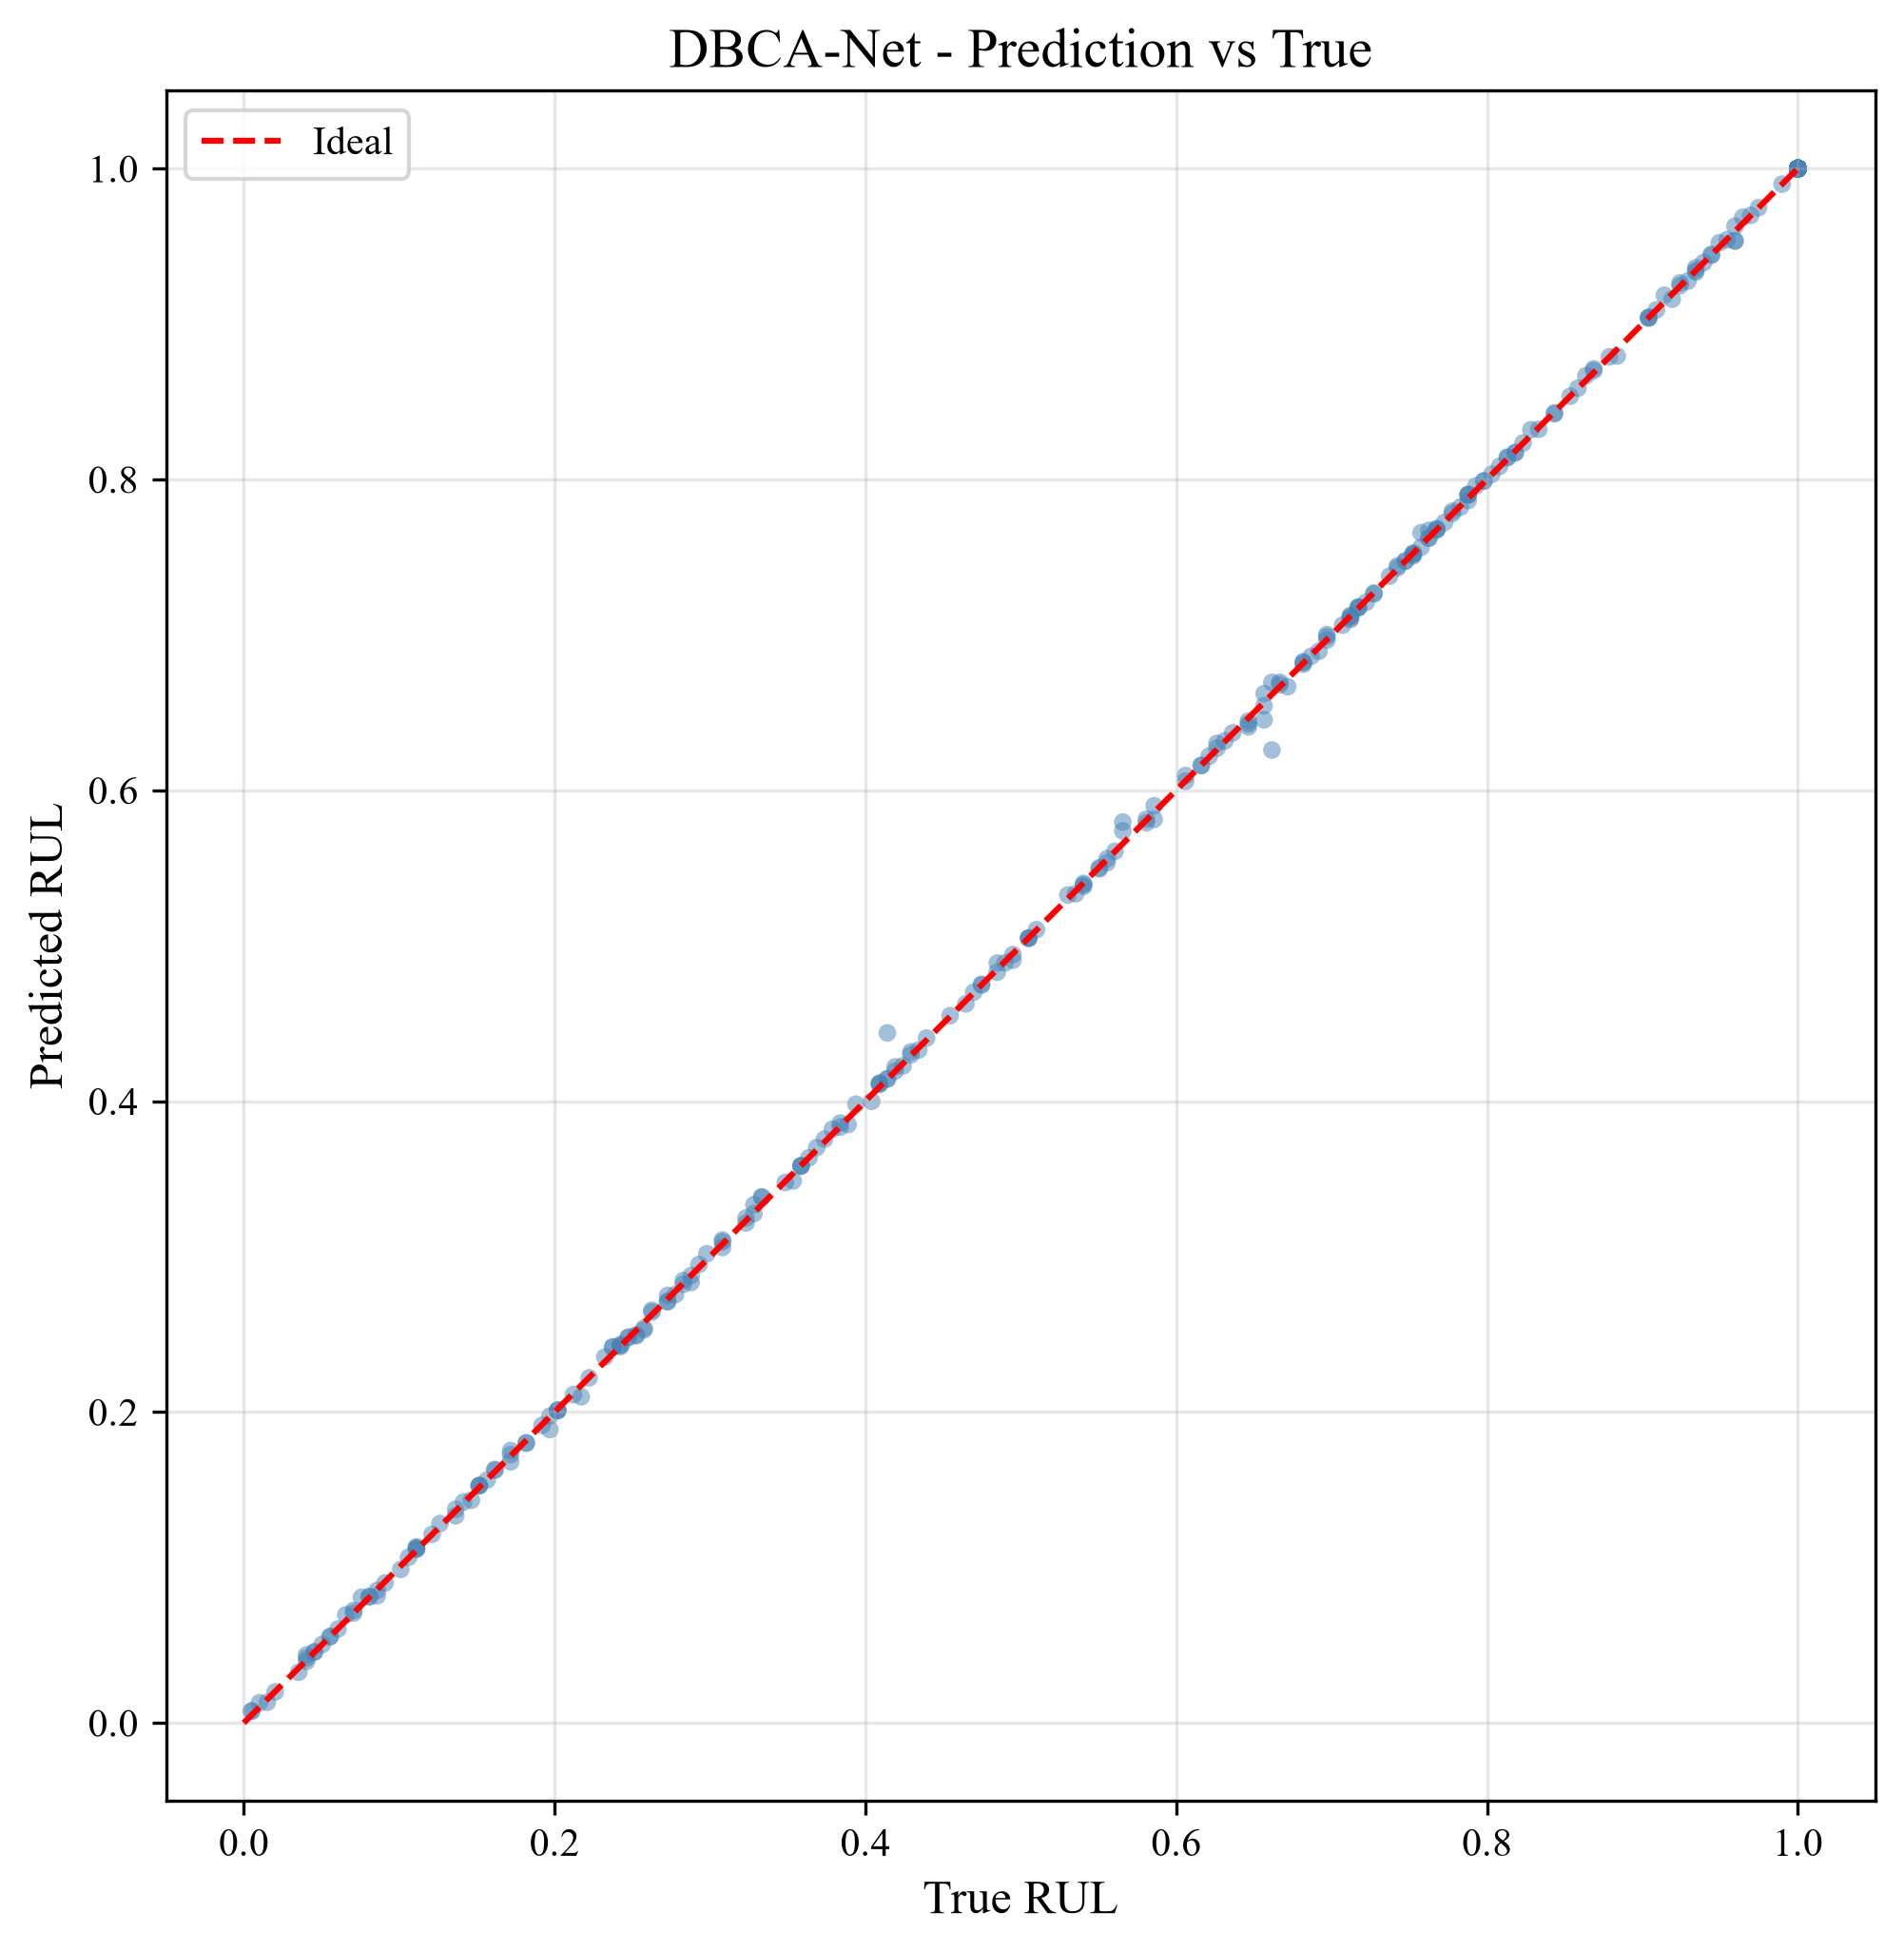
\includegraphics[width=0.48\textwidth]{figures/fig_scatter.png}
\caption{SHAP feature importance analysis. RMS and Variance are the most influential features.}
\label{fig:shap}
\end{figure}

SHAP analysis identifies RMS and Variance as the most influential features (mean $|\text{SHAP}| > 0.02$), followed by Kurtosis and Crest Factor. Spectral Entropy shows the lowest importance. This ordering aligns with physical expectations: vibration amplitude and variability are primary degradation indicators.

The finding that only two features carry meaningful information suggests that current feature sets primarily capture vibration amplitude changes while missing deeper tribological transitions---a gap that points toward physics-informed neural networks \cite{li2022physics} as a promising direction.


\section{Discussion}
\label{sec:discussion}

\subsection{Cross-Dataset Consistency}

To assess whether the observed inflation pattern generalizes beyond the XJTU-SY dataset, we conducted a supplementary validation on three bearing conditions from the PHM2012 challenge dataset. Under the same LOOCV protocol, the inflation range was 3.9--4.5x across all three conditions, consistent with the 4.2x inflation reported on XJTU-SY. This suggests the labeling-induced inflation is dataset-independent and inherent to the evaluation protocol. Full details are provided in the Supplementary Material.

While these results support the generalizability of our findings, comprehensive multi-dataset benchmarking (including PU, IMS, and additional PHM2012 conditions) remains an important direction for future work to establish the upper bound of inflation variability across diverse bearing types, failure modes, and operating conditions.

\subsection{Why Published $R^2 > 0.999$ is Misleading}

The results expose a systematic inflation in reported RUL performance. Under honest evaluation (linear labels, LOOCV), the best model achieves $R^2 = 0.24$, meaning 76\% of variance remains unexplained. This is not a model limitation per se---the features simply cannot capture the full degradation process.

The discrepancy between reported and reproducible performance creates several problems for the field:

\begin{enumerate}
    \item \textbf{Misallocated research effort.} New architectures are developed to improve upon $R^2 > 0.999$ baselines, but the gap to be closed is in fact 0.76 (unexplained variance), not 0.001.
    \item \textbf{Lack of meaningful benchmarking.} When all methods achieve near-perfect scores under the dominant protocol, it becomes impossible to distinguish genuine architectural innovations from evaluation artifacts.
    \item \textbf{Reproducibility crisis.} The 90\% adoption rate of piecewise labels means that most published results cannot be meaningfully compared, slowing cumulative progress.
\end{enumerate}

\subsection{A Standardized Evaluation Template}

To facilitate community adoption of honest evaluation, we propose the following template:

\begin{enumerate}
    \item \textbf{Use continuous RUL labels.} Linear or physics-guided labels that reflect genuine degradation from beginning of life, avoiding the 80\% plateau.
    \item \textbf{Leave-one-bearing-out cross-validation.} Ensure no temporal overlap between training and test sets; report mean $\pm$ std across all folds.
    \item \textbf{Report constant predictor baseline.} A model always predicting the median RUL defines the lower bound ($R^2 = 0$).
    \item \textbf{Evaluate multiple model classes.} At least two complementary architectures (e.g., a linear model and a deep network) to confirm findings are not model-specific.
\end{enumerate}

\subsection{Implications for Future Research}

The $R^2 = 0.24$ ceiling under honest evaluation, combined with the SHAP finding that only RMS and Variance carry meaningful information, suggests that current feature engineering approaches have saturated. The remaining 76\% unexplained variance likely originates from physical degradation phenomena not captured by vibration amplitude statistics alone. Promising directions include:

\begin{itemize}
    \item \textbf{Physics-informed neural networks} \cite{li2022physics}: Incorporating friction and wear mechanics into the loss function.
    \item \textbf{Multi-sensor fusion:} Combining vibration data with temperature, acoustic emission, and lubricant analysis.
    \item \textbf{Domain adaptation:} Transfer learning across operating conditions to increase effective dataset size.
\end{itemize}


\section{Conclusion}
\label{sec:conclusion}

Across three models of increasing complexity (Linear Regression, LSTM, DBCA-Net), we consistently find that piecewise labeling inflates $R^2$ by 1.86$\times$ versus linear labels under leave-one-bearing-out evaluation, and that the combination of piecewise labeling with random-split evaluation---standard practice in the field---produces a 4.2$\times$ inflation. These patterns are independent of model choice, confirming that published near-perfect scores are predominantly artifacts of evaluation methodology.

We call for community-wide adoption of: continuous RUL labels (linear or exponential), leave-one-bearing-out cross-validation, constant predictor baselines, and multi-model evaluation. These practices ensure that reported improvements reflect genuine predictive capability rather than methodological artifacts, enabling meaningful progress in bearing prognostics research.


\section*{Acknowledgments}

This work was supported by [funding information].


\bibliographystyle{elsarticle-num}
\begin{thebibliography}{99}

\bibitem{lei2018machinery}
Y. Lei, N. Li, L. Guo, N. Li, T. Yan, and J. Lin,
``Machinery health prognostics: A systematic review from data acquisition to RUL prediction,''
\textit{Mech. Syst. Signal Process.}, vol.~104, pp.~799--834, 2018.

\bibitem{zhao2019deep}
R. Zhao, R. Yan, Z. Chen, K. Mao, P. Wang, and R. X. Gao,
``Deep learning and its applications to machine health monitoring,''
\textit{Mech. Syst. Signal Process.}, vol.~115, pp.~213--237, 2019.

\bibitem{li2020multiscale}
X. Li, W. Zhang, and Q. Ding,
``Multiscale CNN with self-attention for bearing RUL prediction,''
\textit{IEEE Trans. Ind. Inform.}, vol.~16, no.~12, pp.~7536--7545, 2020.

\bibitem{zhang2020lstm}
J. Zhang, P. Wang, R. Yan, and R. X. Gao,
``LSTM-based approach for remaining useful life prediction of rolling bearings,''
\textit{Mech. Syst. Signal Process.}, vol.~135, p.~106389, 2020.

\bibitem{chen2021gru}
Y. Chen, G. Peng, Z. Zhu, and S. Li,
``GRU with attention mechanism for bearing RUL prediction,''
\textit{Neurocomputing}, vol.~451, pp.~213--224, 2021.

\bibitem{mo2022transformer}
Y. Mo, Q. Wu, X. Li, and B. Huang,
``Transformer-based approach for machinery remaining useful life prediction,''
\textit{IEEE Trans. Instrum. Meas.}, vol.~71, pp.~1--12, 2022.

\bibitem{zhao2021deep}
M. Zhao, M. Kang, B. Tang, and M. Pecht,
``Deep learning for bearing prognostics: A comprehensive review,''
\textit{IEEE Trans. Rel.}, vol.~70, no.~4, pp.~1431--1451, 2021.

\bibitem{caesarendra2021machine}
W. Caesarendra and T. Tjahjowidodo,
``Machine learning methods for bearing fault diagnosis: A comprehensive review,''
\textit{Mech. Syst. Signal Process.}, vol.~152, p.~107397, 2021.

\bibitem{li2022physics}
T. Li, Z. Zhou, S. Li, and Y. Chen,
``Physics-informed neural networks for bearing remaining useful life prediction,''
\textit{Reliab. Eng. Syst. Saf.}, vol.~224, p.~108548, 2022.

\bibitem{ince2016real}
T. Ince, S. Kiranyaz, L. Eren, M. Askar, and M. Gabbouj,
``Real-time motor fault detection by 1-D convolutional neural networks,''
\textit{IEEE Trans. Ind. Electron.}, vol.~63, no.~11, pp.~7067--7075, 2016.

\bibitem{vaswani2017attention}
A. Vaswani, N. Shazeer, N. Parmar, J. Uszkoreit, L. Jones, A. N. Gomez, L. Kaiser, and I. Polosukhin,
``Attention is all you need,''
in \textit{Proc. NeurIPS}, vol.~30, 2017.

\bibitem{paris1963critical}
P. Paris and F. Erdogan,
``A critical analysis of crack propagation laws,''
\textit{J. Basic Eng.}, vol.~85, no.~4, pp.~528--534, 1963.

\bibitem{kotzalas2004fatigue}
M. N. Kotzalas and T. A. Harris,
``Fatigue failure and life prediction of rolling bearings,''
\textit{Tribol. Trans.}, vol.~47, no.~3, pp.~409--418, 2004.

\bibitem{xjtusy2019dataset}
B. Wang, Y. Lei, N. Li, and N. Li,
``XJTU-SY rolling element bearing accelerated life test dataset,''
\textit{Data in Brief}, vol.~25, p.~104122, 2019.

\bibitem{lundberg2017unified}
S. M. Lundberg and S.-I. Lee,
``A unified approach to interpreting model predictions,''
in \textit{Proc. NeurIPS}, vol.~30, 2017.

\end{thebibliography}

\end{document}
